\section{Data and representation}
% Original presentation frame 6
\begin{frame}[t,shrink=5]{The 6D learning set contains 2048 paired full-lattice Xsuite trajectories with fixed splits}
\begin{columns}[T,onlytextwidth]
\begin{column}{0.62\textwidth}
\begin{block}{Reproducible generation chain}
FCC-ee HEB MAD-X optics $\to$ cpymad/Xtrack $\to$ PyWIT wake/impedance $\to (Z_{\rm in},\mu,Z_{\rm out})$.
\[\mathcal D_{\rm track}=\left\{\left(Z_{\rm in}^{(s)},\mu^{(s)},Z_{\rm out}^{(s)}\right)\right\}_{s=1}^{2048}.\]
$10^6$ particles in the recorded timing, and retains 4096 macroparticles in each stored cloud.
\end{block}
\begin{block}{Scope}
The dataset is a fixed archive of 2048 paired trajectories. The training, validation and test splits are also fixed.
\end{block}

\end{column}
\begin{column}{0.36\textwidth}
\begin{block}{Fixed archive}
\begin{center}\begin{adjustbox}{max width=\linewidth}
\begin{tabular}{lr}\toprule Total & 2048\\\midrule Train & 1640\\Validation & 204\\Test & 204\\Retained particles/cloud & 4096\\\bottomrule\end{tabular}
\end{adjustbox}\end{center}
\end{block}

\end{column}
\end{columns}

\sources{\parencite{fcc2026lattice,iadarola2023xsuite,impedan2026pywit,martinez2026code,martinez2026dataset}.}

\end{frame}

% Original presentation frame 7
\begin{frame}[t,shrink=5]{The pipeline separates sampled 6D shape from the physical position and scale of the beam}
\begin{center}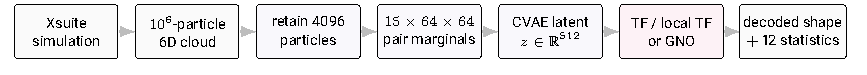
\includegraphics[width=\linewidth,height=25mm,keepaspectratio]{beam_surrogate_pipeline.pdf}\end{center}\begin{columns}[T,onlytextwidth]
\begin{column}{0.49\textwidth}
\begin{block}{Compression and representation}
A direct $64^6$ density grid is infeasible. Fifteen pairwise marginals retain measurable non-Gaussian cores, tails and two-coordinate correlations while allowing convolutional compression.
\end{block}

\end{column}
\begin{column}{0.49\textwidth}
\begin{block}{Phase-space tomography}
Low-dimensional projections are the observables from which high-dimensional beam distributions are inferred. As such the decompression is not unique, but can be trained to preserve the measured marginals and the known physical statistics.
\end{block}

\end{column}
\end{columns}

\sources{\parencite{goutierre2023physics,hoover2024tomography,roussel2023reconstruction}.}

\end{frame}

% Original presentation frame 8
\begin{frame}[t,shrink=5]{The CVAE compresses projected shape while conditioning keeps known beam information explicit}
\begin{columns}[T,onlytextwidth]
\begin{column}{0.49\textwidth}
\begin{block}{Conditional statistics match the known beam information}
\begin{itemize}
\item Direct propagation of $15\times64\times64=61,440$ bins is expensive.
\item A stochastic latent state gives a continuous, sampleable representation of projected shape.
\item Explicit conditioning retains known statistics and domain variables, posterior sampling enables the later sensitivity study.
\end{itemize}
\end{block}

\end{column}
\begin{column}{0.49\textwidth}
\begin{center}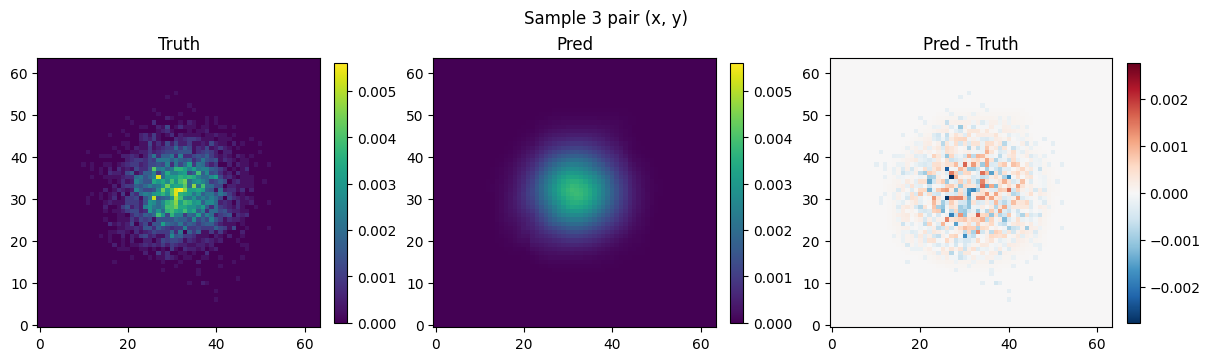
\includegraphics[width=\linewidth]{cvae_reconstruction_xy.png}\end{center}\begin{center}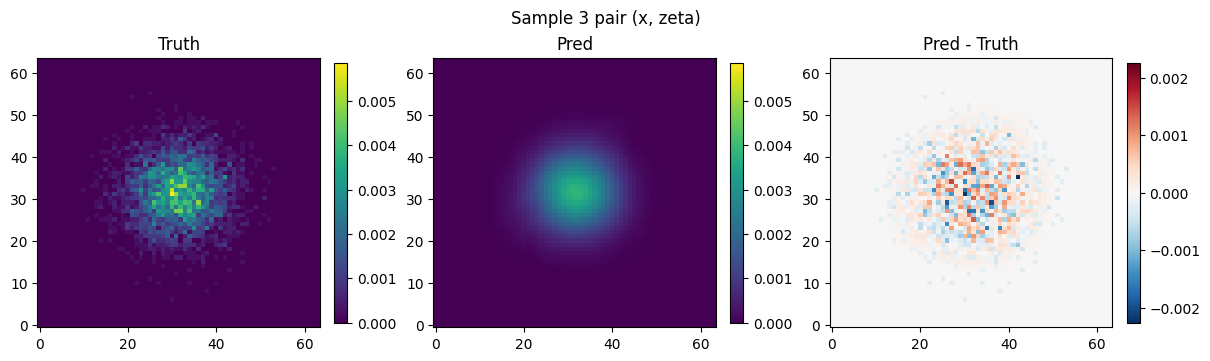
\includegraphics[width=\linewidth]{cvae_reconstruction_xzeta.png}\end{center}
\end{column}
\end{columns}

\sources{\parencite{kingma2014vae,sohn2015cvae}.}

\end{frame}

% Original presentation frame 9
\begin{frame}[t,shrink=5]{The CVAE is a stochastic encoder-decoder that learns a posterior distribution over a latent space}
\begin{columns}[T,onlytextwidth]
\begin{column}{0.49\textwidth}
\begin{block}{Probabilistic motivation for the CVAE}
\begin{itemize}
\item A deterministic autoencoder predicts a single realization, the CVAE learns $q_\phi(z\mid H,c,\mu)$.
\item Conditioning $c=[\sigma,m]$ keeps known scale, centroid and domain information explicit.
\item The sampleable 512-state can be propagated by Transformer or neural operators and later resampled for latent-sensitivity analysis.
\end{itemize}
\end{block}
\begin{block}{Implemented posterior and objective}
\[q_\phi(z\mid H,c,\mu)=\mathcal N(m_z[\mu],\operatorname{diag}\sigma_z^2),\]
\[z=m_z[\mu]+\sigma_z\odot\epsilon,\quad\epsilon\sim\mathcal N(0,I).\]
\scriptsize The prior is fixed, the encoder learns $m_z$ and $\sigma_z^2$. Reparameterization keeps sampling differentiable.
\end{block}

\end{column}
\begin{column}{0.49\textwidth}
\begin{center}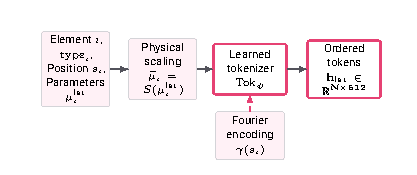
\includegraphics[width=\linewidth]{lattice_tokenization.pdf}\end{center}\begin{block}{Lattice tokenization}
The CVAE compresses beam shape to $z_0$, while the tokenizer retains lattice order and local physical descriptors through $\{h_i\}_{i=1}^{N}$.
\end{block}

\end{column}
\end{columns}

\sources{\parencite{wang2026latent,kingma2014vae,sohn2015cvae}.}

\end{frame}

